\documentclass{article}
\usepackage{cite}
%Para revisar el doc
\usepackage[colorinlistoftodos]{todonotes}

%Configuraciones para el español 
\usepackage[spanish,es-tabla]{babel}
\selectlanguage{spanish}
\usepackage[utf8]{inputenc}
\spanishdecimal{.}

%Para autores
\usepackage{authblk}

%Configuraciones para las ecuaciones 
\usepackage{amsmath}

%Configuraciones las gráficas o tablas
\usepackage{graphicx}
\usepackage{subcaption}
\usepackage{eso-pic}
\usepackage{multirow} 

%Configuraciones para hipervínculos del texto
\usepackage[hidelinks]{hyperref}

%Configuraciones figuras
\usepackage{graphicx} %Figuras
\usepackage{float} %Figuras

%Configuraciones para citar apa 
\usepackage{apacite}

%Para unir varias filas y columnas
\usepackage{multirow}
\usepackage{multicol}

%Para adicionar comentarios qeu salgan en el pdf
\usepackage[colorinlistoftodos]{todonotes}

%Configuración de la geometría de la hoja
\usepackage[paperwidth=16.5cm, paperheight=23cm, left=1.8cm, right=1.8cm, bottom=3cm, textheight=17.5cm, top=2cm]{geometry}

%Configuración del url 
\usepackage[hyphens]{url}

%Configuración de tablas
\usepackage{longtable}

%Para crear un segundo título
% \usepackage{titling}
% \title{Some Title}

%Tablas con ancho definido
\usepackage{array}
\newcolumntype{M}{>{\centering\arraybackslash}m{1.45cm}}
\newcolumntype{A}{>{\centering\arraybackslash}m{1cm}}
\newcolumntype{C}{>{\centering\arraybackslash}m{2.8cm}}

%Para arreglar la disposición de las imágenes
\renewcommand{\topfraction}{.85}
\renewcommand{\bottomfraction}{.7}
\renewcommand{\textfraction}{.15}
\renewcommand{\floatpagefraction}{.66}
\renewcommand{\dbltopfraction}{.66}
\renewcommand{\dblfloatpagefraction}{.66}
\setcounter{topnumber}{9}
\setcounter{bottomnumber}{9}
\setcounter{totalnumber}{20}
\setcounter{dbltopnumber}{9}

%Para crear un subsubsubsection
\usepackage{titlesec}
\setcounter{tocdepth}{5} %Para que se muestre en la tabla de contenidos

\setcounter{secnumdepth}{4}
\titleformat{\paragraph}
{\normalfont\normalsize\bfseries}{\theparagraph}{1em}{}
\titlespacing*{\paragraph}
{0pt}{3.25ex plus 1ex minus .2ex}{1.5ex plus .2ex}

\setcounter{secnumdepth}{5}
\titleformat{\subparagraph}
{\normalfont\normalsize\bfseries}{\thesubparagraph}{1em}{}
\titlespacing*{\subparagraph}
{0pt}{3.25ex plus 1ex minus .2ex}{1.5ex plus .2ex}



\title{ \Large \bf GEOHAZARD: base de datos por movimientos en masa y avenidas torrenciales en Colombia y el departamento de Antioquia}

%Autores
\author[]{Edier Aristizábal\thanks{evaristizabalg@unal.edu.co}}
\author[]{Daniel Correa\thanks{dcorreaz@unal.edu.co}}
\author[]{Ana Maria Valencia\thanks{anvalencial@unal.edu.co}}
\author[]{Carolina Garcia\thanks{cargarcia@unal.edu.co}}
\author[]{Erluan Zabaleta\thanks{ezabaleta@unal.edu.co}}

\affil[]{Departamento de Geociencias y Medio Ambiente, Universidad Nacional de Colombia}

\date{}

\begin{document}
\maketitle

\section*{Abstract}
Colombia is a country characterized by its geographical diversity and high vulnerability to natural hazards such as landslides, flash floods, earthquakes, volcanic activity, hurricanes, and tsunamis. The convergence of tectonic plates and its mountainous topography significantly increase the risk of natural disasters. This article presents an analysis of natural disaster events in Colombia through the development of a web application called Geohazard, which allows for the visualization and analysis of a database of landslides and debris flows in Colombia. The application integrates data from various sources, including DesInventar and SIMMA, providing a valuable resource for disaster risk management. The spatial and temporal patterns of these phenomena, as well as their impact in terms of fatalities and material damage, are analyzed. The results show a spatial concentration of these events in the mountainous areas of the Andes and a temporal cycle related to the rainy seasons. This work highlights the importance of having systematized historical records to implement effective mitigation measures and reduce vulnerability to natural disasters in Colombia.
\par Keywords: GEOHAZARD, landslides, debris flow, databases, Colombia, Antioquia.

\section*{Resumen}
Colombia es un país caracterizado por su diversidad geográfica y su alta vulnerabilidad a amenazas naturales, tales como movimientos en masa, avenidas torrenciales, sismos, actividad volcánica, huracanes y tsunamis. La convergencia de placas tectónicas y su topografía montañosa son factores que incrementan significativamente el riesgo de desastres por fenómenos naturales. Este artículo presenta un análisis de los desastres por fenómenos naturales en Colombia a través del desarrollo de un aplicativo web denominado Geohazard, que permite la visualización y análisis de una base de datos de movimientos en masa y avenidas torrenciales en Colombia. El aplicativo integra datos de diversas fuentes, como DesInventar y SIMMA, proporcionando un recurso valioso para la gestión del riesgo de desastres. Se analizan los patrones espaciales y temporales de estos fenómenos, así como su impacto en términos de víctimas fatales y daños materiales. Los resultados muestran una concentración espacial de estos eventos en las zonas montañosas de los Andes y un ciclo temporal relacionado con las temporadas de lluvias. Este trabajo subraya la importancia de contar con registros históricos sistematizados para implementar medidas efectivas de mitigación y reducir la vulnerabilidad ante desastres por fenómenos naturales en Colombia.
\par Palabras claves: GEOHAZARD, deslizamientos, avenidas torrenciales, bases de datos, Colombia, Antioquia.


\section{Introducción}
Colombia está conformado por un territorio diverso, susceptible a una gran diversidad de amenazas naturales \cite{aristizabal2006geomorfologia}. Su ubicación en el trópico la caracterizan por la variabilidad climática y presencia de lluvias durante todo el año, con eventos de corta duración y alta intensidad \cite{poveda2004hidroclimatologia}. El marco tectónico está representado por dos placas oceánicas, Nazca y Caribe, que colisionan con la placa continental Suramericana, dando lugar a la cadena montañosa de los Andes \cite{cediel2003tectonic}. En estos terrenos de altas pendientes es común la ocurrencia de movimientos en masa y avenidas torrenciales \cite{aristizabal2020spatial}.  El continuo desplazamiento y colisión de estas placas tectónicas da lugar a la presencia de fallas geológicas activas que dan lugar a sismos superficiales \cite{taboada2000geodynamics}. Estas placas además de colisionar, subducen bajo la placa suramericana generando material magmático que asciende, y forma una cadena de volcanes activos con erupciones violentas \cite{vasquez2010magmatic}. Las islas y costas sobre el mar Caribe están expuestas a huracanes \cite{ortiz2012exposure}, mientras las islas y costas sobre el océano pacífico están expuestas a tsunamis \cite{otero2014tsunami}. Las tierras bajas y llanas del norte del país, de los llanos orientales y la Amazonia, hacia donde drenan los principales ríos, están expuestas a inundaciones \cite{duarte2017identificacion}.

El crecimiento acelerado de la población y su desplazamiento hacia zonas urbanas ha aumentado la exposición humana e infraestructura a dichas amenazas de origen natural, conformando escenarios de riesgo que recurrentemente se materializan en desastres \cite{aristizabal2020spatial}. Casos como Armero en 1985, donde aproximadamente 23 mil personas perdieron la vida por una avenida torrencial de origen volcánico \cite{hermelin2005desastres}; Villatina en 1987, donde un deslizamiento en la ciudad de Medellín generó la muerte de aproximadamente 500 personas \cite{garcia20055}; y el caso reciente de Mocoa en 2017, donde intensas lluvias en la parte alta de las cuencas montañosas, generaron un enjambre de movimientos en masa que formaron una avenida torrencial, la cual se propagó a largo de los principales ríos que cruzan la ciudad destruyendo cientos de viviendas con un total de 330 víctimas \cite{garcia2019dynamic}.

Y aunque los desastres por fenómenos de origen natural son recurrentes en Colombia, no existe una base de datos que compile de forma sistemática y homogénea estos eventos. Los registros históricos son una herramienta fundamental para el análisis de desastres e implementación de medidas de mitigación. Proporciona información espacial y temporal sobre la extensión geográfica, la incidencia y generalmente pérdidas humanas y económicas \cite{gomez2023spatial}.

Algunos intentos de registros históricos han sido realizados. El proyecto con mayor éxito probablemente ha sido el Sistema de Inventario de Efectos de Desastres, denominado Desinventar, y desarrollado en el año 1994 por La Red de Estudios Sociales en Prevención de Desastres LA RED, la Corporación Observatorio Sismológico del Suroccidente Colombiano (OSSO), y la Oficina de la Naciones Unidas para la Reducción del Riesgo de Desastres (UNISDR). El DesInventar era un software que permitía la sistematización, organización, recolección y visualización de los desastres históricos y el análisis de estos desde un punto de vista espacial agregado y temporal \cite{marulanda2010revealing}. Se implementó en más de 20 países convirtiéndose una fuente importante de consulta para el análisis de la gestión del riesgo de desastres. El manejo y desarrollo del DesInventar en Colombia estuvo a cargo de la OSSO. En Colombia se crearon 12 bases de datos para diferentes regiones y ciudades del país y una a nivel nacional con registros de desastres ocurridos desde el año 1900. Para el departamento de Antioquia y el Valle de Aburrá se construyeron dos bases de datos individuales y actualizadas que fueron elaboradas por la Universidad EAFIT, el Departamento Administrativo de Gestión del Riesgo de Desastres de la ciudad de Medellín (DAGRD), el Área Metropolitana del Valle de Aburrá (AMVA), el Departamento Administrativo para la Prevención, Atención y Recuperación de Desastres (DAPARD) y trabajos anteriores como \citeA{saldarriaga2003compilacion} y \citeA{polanco2005compilacion}. El DesInventar (\url{https://www.desinventar.net/}) se transformó a una herramienta web implementada para algunos países en el mundo, entre ellos Colombia. 

Existen otras bases de datos a nivel mundial que compilan la ocurrencia de desastres donde resalta EM-DAT, mantenido por el Centro de Investigación sobre Epidemiología de Desastres (CRED) en la Escuela de Salud Pública de la Université catholique de Louvain ubicada en Bruselas, Bélgica \cite{guha2002quality}. Esta base de datos contiene registros sobre la ocurrencia y los efectos de más de 17.000 desastres por fenómenos de origen natural y tecnológico que en el mundo desde 1900 hasta la actualidad.

Para el caso de movimientos en masa en Colombia existe la base de datos SIMMA (\url{https://simma.sgc.gov.co/}) del Servicio Geológico Colombiano, el cual lo define como un sistema que permite cargar, administrar y consultar de forma abierta los movimientos en masa ocurridos en Colombia.

En este trabajo se presenta el aplicativo web denominado Geohazard (\url{https://geohazards.com.co/visor-geohazard.html}), en el cual existen dos bases de datos de desastres generados por fenómenos naturales tipo movimientos en masa y avenidas torrenciales. La primera de ellas para todo el territorio colombiano, donde se registran eventos fatales, es decir que registraron al menos una persona fallecida, y la segunda para el departamento de Antioquia, donde se registran todos aquellos eventos que registran algún nivel de afectación a infraestructura o perdidas humanas. Esta base de datos es construida y alimentada continuamente por el semillero Geohazard (\url{https://geohazards.com.co}) de la Universidad Nacional de Colombia, sede Medellín.

\section{GEOHAZARD: aplicativo web}
El aplicativo web trata de un visor cartográfico desarrollado con tecnologías como HTML, CSS y JavaScript. Está implementado con la librería de código abierto Leaflet para la gestión de mapas, alojado en GitHub pages y utiliza la base de datos proporcionada por la plataforma Firebase de Google para almacenar y acceder a los registros.

\begin{figure}[ht!]
    \centering
      {\includegraphics[width=1\textwidth]{Figuras/visor_general.png}}
    \caption{Interfase del aplicativo web de consulta de la base de datos GEOHAZARD (\url{https://geohazards.com.co})}
    \label{fig:app}
\end{figure}

Además de proporcionar una interfaz intuitiva y fácil de usar, el aplicativo ofrece una serie de funcionalidades destinadas a facilitar la exploración y el análisis de la información. Entre estas funcionalidades, dispuestas en la barra lateral del aplicativo, se incluyen la elección de mapas base, el filtrado y la visualización de eventos, análisis estadísticos de los eventos presentes en el mapa, la visualización de información de estaciones de campo realizadas en el marco de diferentes proyectos, la carga de información externa en formatos Shapefile, GeoJSON, KML, KMZ y TIF, así como la descarga de eventos en formatos Shapefile y GeoJSON. Además, cuenta con una sección para agregar, editar y eliminar eventos, lo que contribuye a la actualización y enriquecimiento continuo de la base de datos.

Al acceder al aplicativo, los usuarios pueden visualizar automáticamente todos los registros de eventos de desastres fatales por movimientos en masa y avenidas torrenciales registrados en la base de datos de Colombia. La información detallada de cada evento está disponible al seleccionar en el marcador correspondiente en el mapa. Además, los usuarios pueden filtrar los eventos según una variedad de parámetros, como la base de datos (Colombia o Antioquia), el rango de fechas, el departamento o subregión, la ciudad, el tipo de evento, el detonante y el número de fallecidos. Una vez completada la búsqueda, los eventos que cumplan con los criterios seleccionados se presentan en pantalla para su revisión y posterior descarga.

Todos los registros cuentan con los siguientes campos: longitud, latitud, fecha de ocurrencia, tipo de fenómeno, departamento o subregión, municipio, vereda, sitio, incertidumbre en la localización del evento, factor detonante, número de fallecidos, pérdidas económicas, fuente de los datos, notas adicionales.

La aplicación cuenta con una pestaña con gráficos de las consultas realizadas. Esta sección se ha diseñado para mejorar la comprensión de los datos y facilitar los análisis estadísticos de los eventos. Se trata de un conjunto de gráficos generados a partir de los eventos presentes en pantalla, tanto para la base de datos de Colombia, como la de Antioquia, así como cualquier tipo de filtrado que realice el usuario.

Entre los gráficos generados, se incluyen los siguientes agrupamientos de datos: el total de registros y fallecidos según el tipo de evento, el porcentaje de registros según el detonante, el total de eventos por año y el total de eventos por mes. Estos gráficos son interactivos y permiten al usuario visualizar los datos detallados al pasar el cursor sobre ellos. Además, los gráficos pueden ser exportados como imágenes en formato \textit{PNG}.

\begin{figure}[ht!]
  \begin{minipage}{.48\linewidth}
    \centering
      {\includegraphics[width=1\textwidth]{Figuras/graficos_1_2_col.png}}
  \end{minipage}\quad
  \begin{minipage}{.48\linewidth}
    \centering
      {\includegraphics[width=1\textwidth]{Figuras/graficos_3_4_ant.png}}
  \end{minipage}
    \caption{Gráficas generadas a partir de los eventos en pantalla (A) Gráficas de total de registros y fallecidos según el tipo de evento y porcentaje de eventos según detonante para la base de datos de Colombia, (B) Gráficas de total de eventos por año y total de eventos por mes para la base de datos de Antioquia}
    \label{fig:data}
\end{figure}


\section{Construcción de la base de datos}
La base de datos GEOHAZARD ha sido construida basada en la base de datos DesInventar. Para esto se agruparon la base de datos a nivel Colombia, con las 12 bases de datos que existían a nivel regional y su depuración para eliminar eventos repetidos. Posteriormente se incluyeron los eventos reportados en la base de datos SIMMA.

La base de datos se actualiza de forma diaria con reportes de los periódicos nacionales y regionales, consultaos en sus paginas web. Adicionalmente se consultan las redes sociales de las entidades que actúan como primero respondientes, tales como Bomberos, Cruz Roja, y las oficinas locales y regionales de gestión del riesgo de desastre.

A partir de los datos suministrados en dichas fuentes se alimenta la base de datos. La localización se realiza mediante coordenadas que se obtienen a partir de las descripciones y utilizando sistemas de información geográfica y herramientas de sensoramiento remoto como Google Earth. En un gran numero de eventos se logra identificar la ubicación del sitio mediante imágenes de satélite, lo cual reduce considerablemente la incertidumbre asociada a la localización, sin embargo existen casos en los cuales solo se tiene disponible la descripción de las fuentes escritas, por lo cual la localización es aproximada. Para esto se creo un campo donde se consigna el nivel de incertidumbre en la localización del evento.

\section{Registros para Colombia}
La Figura \ref{fig:locCol} presenta la localización de los movimientos en masa y avenidas torrenciales para los registros de la base de datos. Al año 2023, la base de datos para Colombia cuenta con 2.415 registros, con un total de 2.259 movimientos en masa que corresponde al 93.5\%  y 156 avenidas torrenciales que representan el restante 6.5\% de los registros. .

\begin{figure}[ht!]
    \centering
      {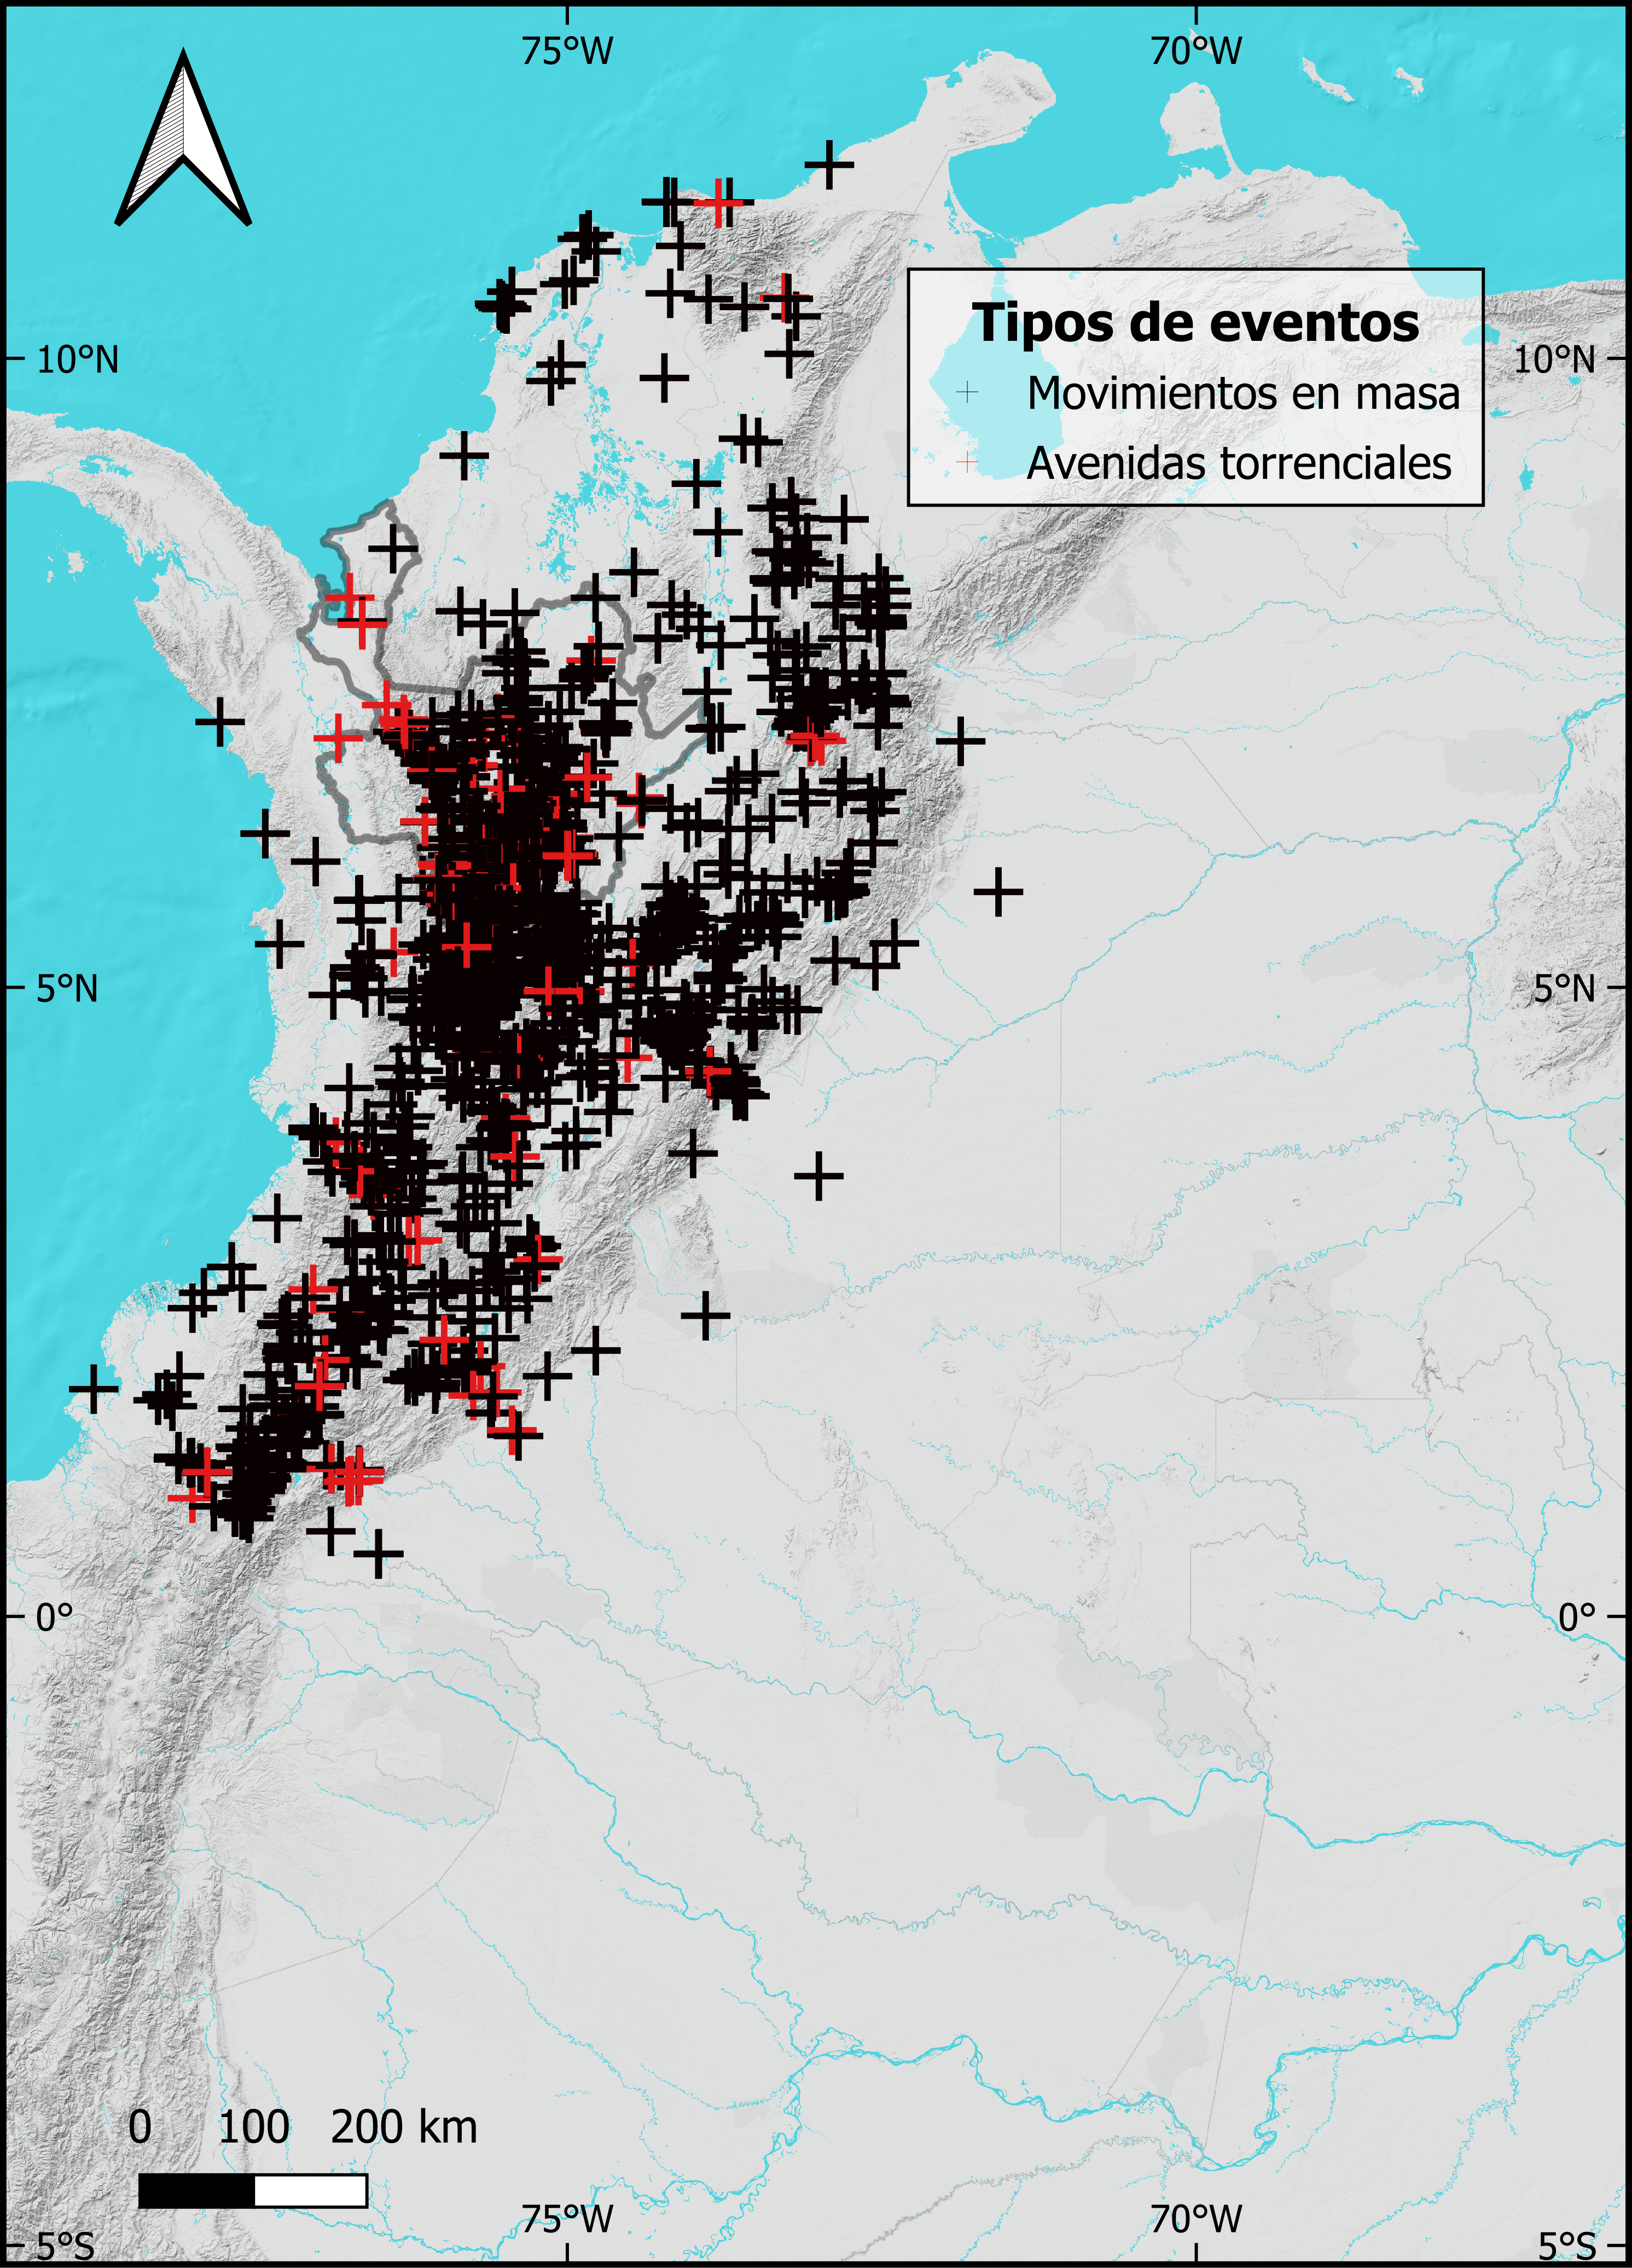
\includegraphics[width=0.6\textwidth]{Figuras/col.png}}
    \caption{Localización de los registros de la base de datos Colombia}
    \label{fig:locCol}
\end{figure}

La Figura \ref{fig:AnualCol} contiene el número de registros reportados por año. Se observa una tendencia creciente exponencial hasta llegar a su máximo en el año 2010, a partir del cual sobresale una fuerte caída en los registros. El primer registro corresponde al 23 de abril de 1880 donde una avenida torrencial en la quebrada La Iguaná en la ciudad de Medellín dejo como saldo 7 personas fallecidas y un número no determinado de daños materiales.

\begin{figure}[ht!]
    \centering
      {\includegraphics[width=0.9\textwidth]{Figuras/anualColombia.png}}
    \caption{Número de registros anuales para Colombia}
    \label{fig:AnualCol}
\end{figure}

En términos de víctimas mortales los movimientos en masa y avenidas torrenciales han dejado un saldo de 34.577 muertos. En contraste, aunque las avenidas torrenciales corresponden a un bajo porcentaje de registros, el número de muertos asciende a 22.877 muertos, que representan el 67\%, mientras los movimientos en masa registran 11.269 muertos, tan solo el 33\%. 

Como factor detonante dominan los casos que registran una causa desconocida (48\%), seguido por la lluvia (37\%), otras causas (11\%) y factor antrópico (3.5\%). Existen otras causas como los sismos y la actividad volcánica con un bajo porcentaje. El departamento mas afectado es Antioquia con el 33.5\% de los movimientos en masa, seguido por Caldas con el 12\% y Risaralda con el 8\%.

\section{Registros para Antioquia}
La Figura \ref{fig:LocAnt} presenta la localización de los registros de la base de datos para el departamento de Antioquia. Las regiones mas afectadas son el Valle de Aburrá con el 44\% de los registros, el suroeste antioqueño con el 16\%, y el oriente con el 12\%. Como factores detonantes domina la lluvia con el 63\% de los registros, seguido por causas desconocidas (30\%), y causas antrópicas con el 5\%.

\begin{figure}[ht!]
    \centering
      {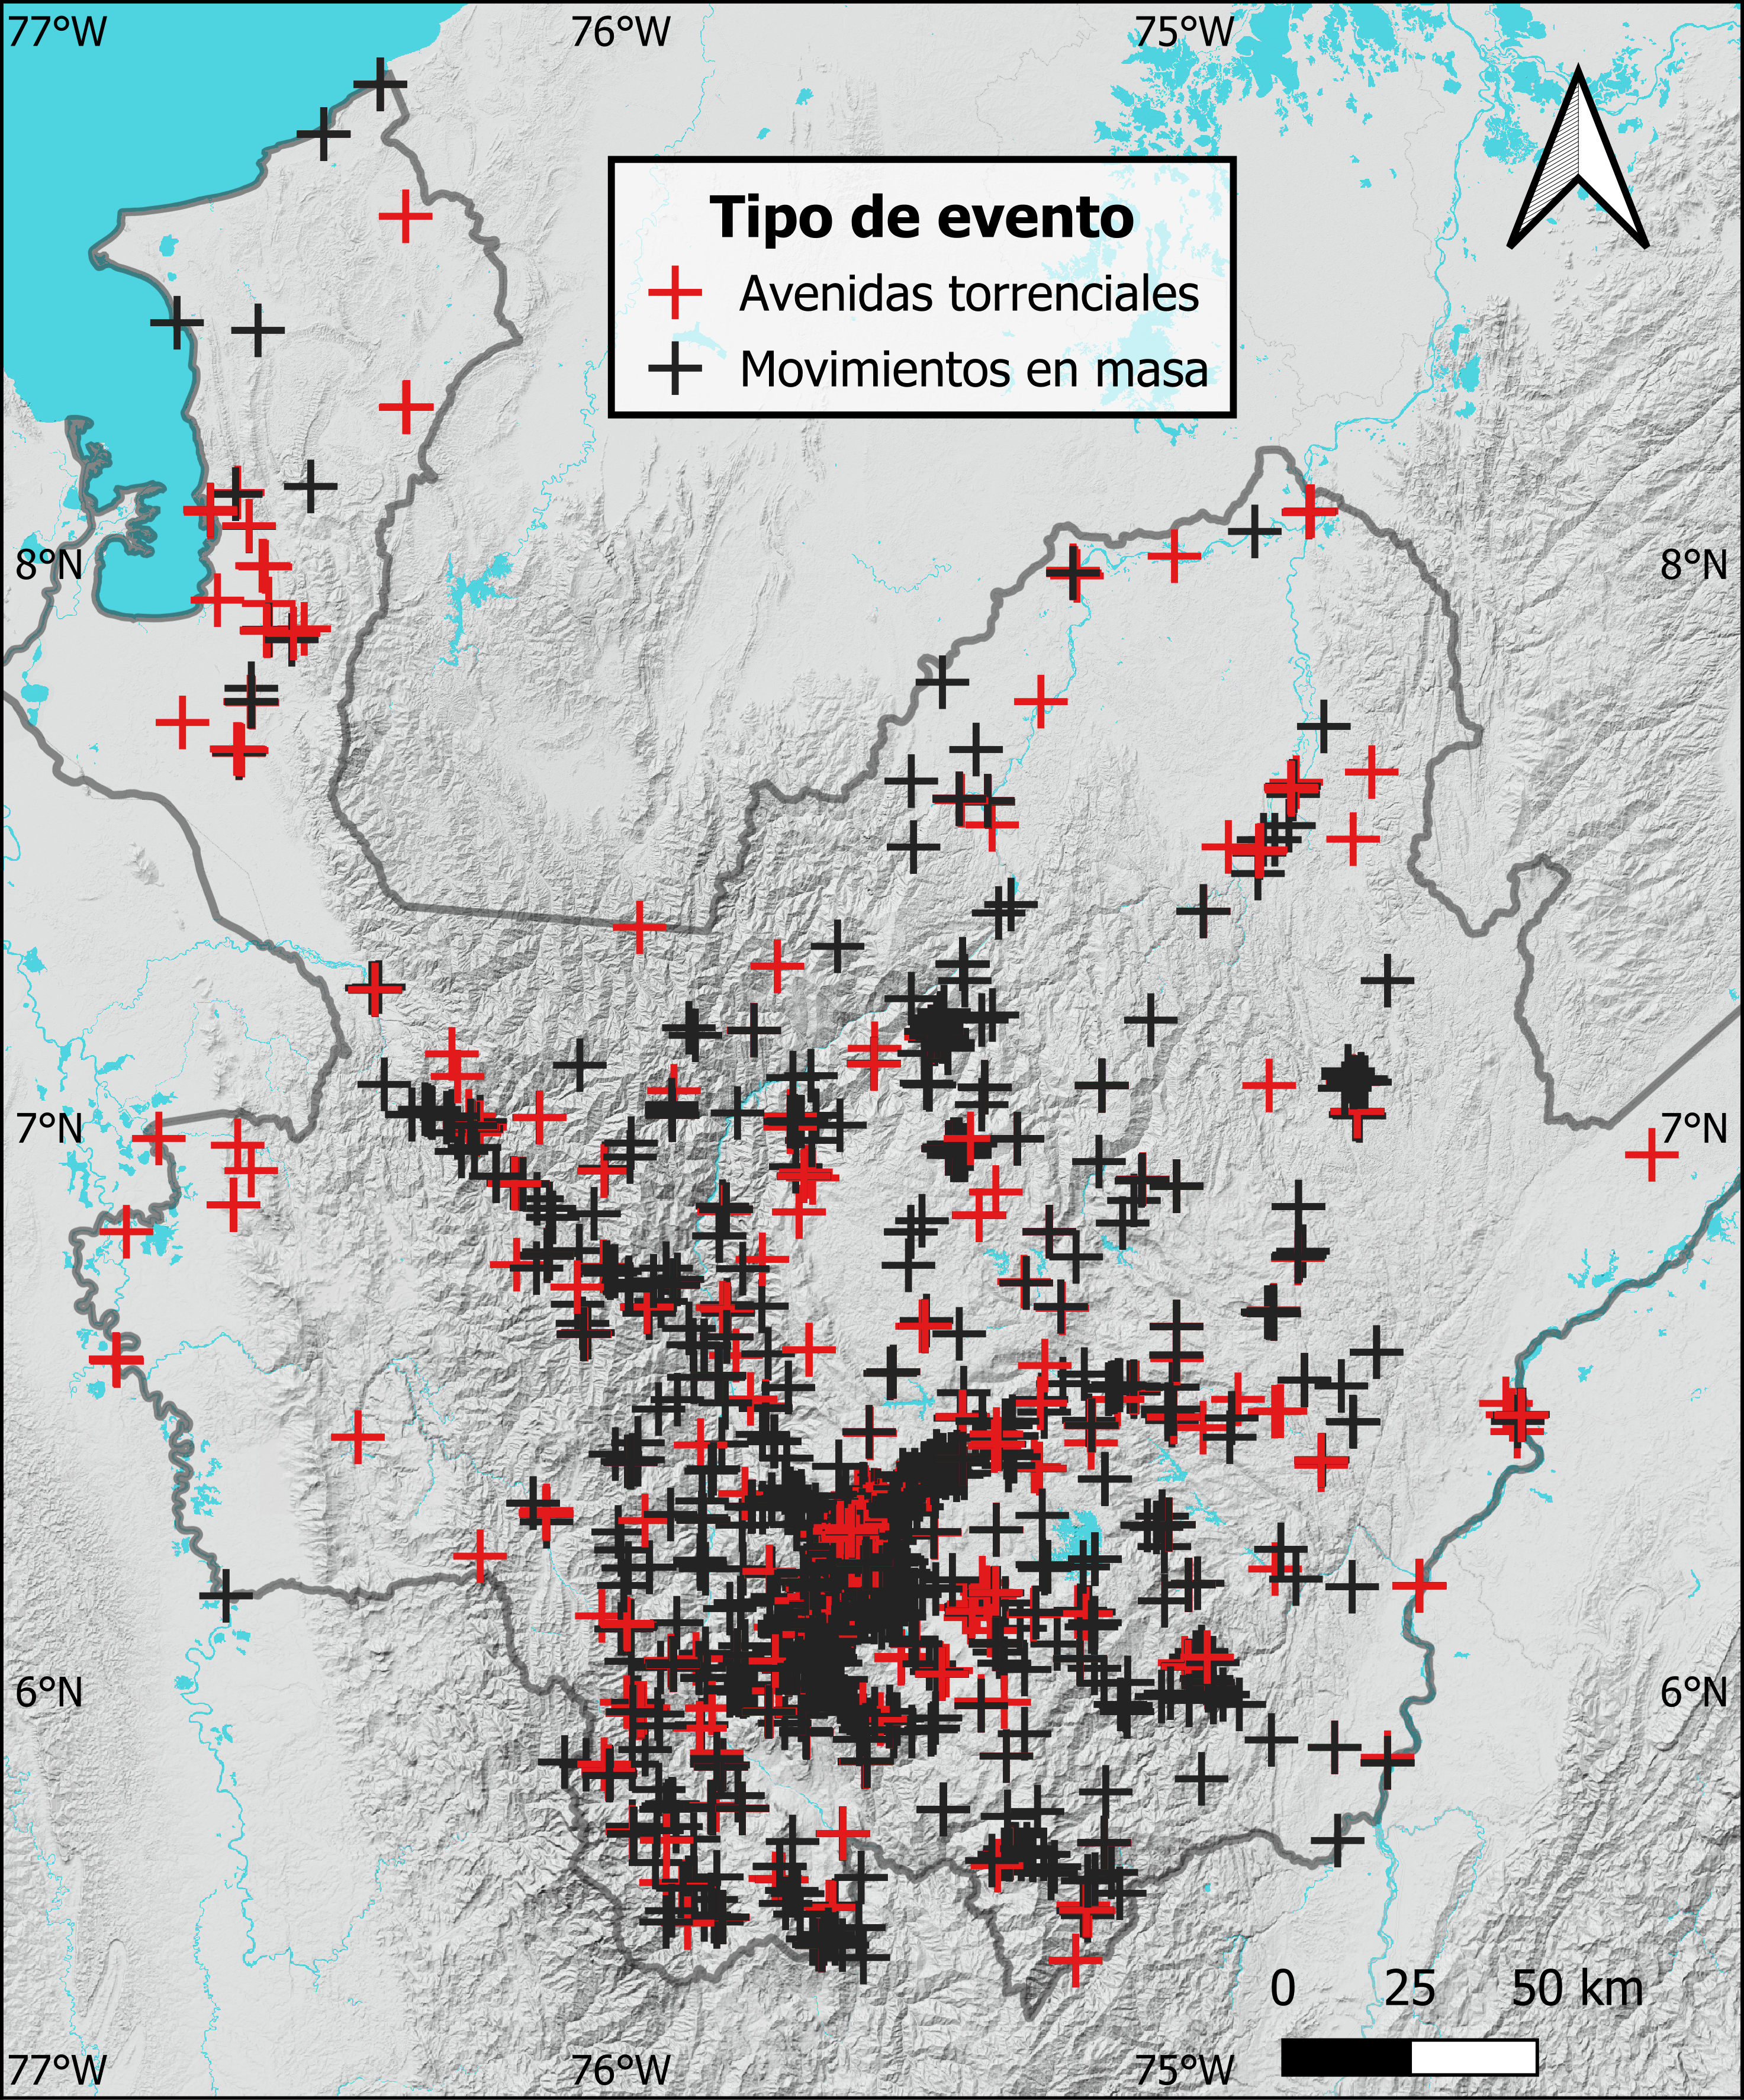
\includegraphics[width=0.6\textwidth]{Figuras/ant.png}}
    \caption{Localización de los registros de la base de datos Antioquia}
    \label{fig:LocAnt}
\end{figure}

La Figura \ref{fig:AnualAnt} presenta el número de registros anuales de la base de datos Antioquia. Al año 2023, la base de datos para Antioquia cuenta con un total de 5.035 registros, donde 3.076 registros corresponden a movimientos en masa (61\%), y 1.959 registros a avenidas torrenciales  (39\%). Del total de eventos solo el 15\% registra víctimas mortales y entre estos el 73\% son movimientos en masa. Es decir, que de forma similar a la base de datos para Colombia, los movimientos en masa son los eventos fatales mas frecuentes, pero en este caso, los movimientos en masa dominan en numero de víctimas con 3.021 muertos (75\%). En la base de datos de Colombia el caso excepcional de Armero cambia esta tendencia.

\begin{figure}[ht!]
    \centering
      {\includegraphics[width=0.9\textwidth]{Figuras/anualAntioquia.png}}
    \caption{eventos de base de datos Antioquia}
    \label{fig:AnualAnt}
\end{figure}

\section{Avenidas torrenciales: fenómenos concatenados con gran capacidad de destrucción}
En la base de datos de Colombia el 64\% de las víctimas fatales están asociados a un solo evento: la avenida torrencial de origen volcánico, fenómeno denominado lahar, registrada el 13 de noviembre de 1985 a lo largo de los ríos Lagunilla, Gualí y Chichiná que dejó como saldo 4.407 viviendas destruidas y 21.559 entre muertos y desaparecidos. Este evento afectó poblaciones de los departamentos del Tolima y Caldas, principalmente los municipios de Armero y Chinchiná.

El segundo evento con mayor número de pérdidas humanas corresponde a la avenida torrencial del río Paez en el departamento del Cauca, el 6 de junio de 1994, con un estimado de 1.100 personas \cite{hermelin2005desastres}. Donde un evento concatenado de lluvias y un sismo de magnitud 6.8 Mw generó un enjambre de movimientos en masa en la cuenca del río Paez. La mayoría de los cuales, por el alto contenido de agua de los suelos, se transformaron en flujos de lodo que alcanzaron el cauce principal del río y dieron lugar a un evento torrencial, que arrasó con toda la infraestructura que encontró en las riveras del río.

En la base de datos, también destaca la avenida torrencial que destruyó parcialmente el municipio de Mocoa (Putumayo), entre la noche del 31 de marzo y 1 de abril de 2017. Donde un evento de lluvia intenso, que superó 130 mm en 3 horas, detonó mas de 600 movimientos en masa, la mayoría de ellos tipo flujos, que alcanzaron los cauces de las cuencas Taruca, Mulato y Sangoyaco, dando lugar a una avenida torrencial que destruyó 130 viviendas y generó la muerte de aproximadamente 330 personas \cite{garcia2019dynamic}.


\begin{longtable}{|>{\raggedright}p{1.4cm}|>{\raggedright}p{2.8cm}|>{\raggedright}p{1.6cm}|>{\raggedright}p{2.5cm}|>{\raggedright\arraybackslash}p{2.5cm}|}
\caption{Avenidas torrenciales y eventos concatenados más fatales en Colombia} \label{tabla_avt} \\
\hline
\textbf{Fecha} & \textbf{Localización} & \textbf{Víctimas} & \textbf{Agua} & \textbf{Sedimentos} \\
\hline
Nov. 24/1979 & El Playón - Santander & 100 & Represamiento & Cauce \\
\hline
Nov. 12/1985 & Armero - Tolima & 21.559 & Fusión parcial del glaciar & Piroclastos y cauce \\
\hline
Jun. 6/1994 & Río Paez & 1.100 & Precipitación larga duración & Sismo y enjambre deslizamientos \\
\hline
May. 17/2015 & Salgar - Antioquia & 104 & Precipitación intensa & Enjambre deslizamientos y cauce \\
\hline
Mar. 31/2017 & Putumayo - Mocoa & 330 & Precipitación intensa & Enjambre deslizamientos y cauce \\
\hline
\end{longtable}


Todos estos eventos tipo avenidas torrenciales, señalados anteriormente, se caracterizan por su naturaleza en cadena que combina diferentes amenazas, su gran capacidad destructiva y la incertidumbre en el registro de víctimas fatales. En todos ellos el número de personas fallecidas no se logró establecer con precisión, debido al volumen de material que involucró cada evento y la extensión de las zonas afectadas. Sin embargo el número de desaparecidos reportados en cada evento hace suponer que las víctimas puede ser mayor.

Las avenidas torrenciales se caracterizan por su naturaleza a escala de cuenca. Es decir que no son eventos que se restringen a lo largo de los cauces, sino que tienen un origen diverso que combina tres elementos: cuencas de montaña, disponibilidad de sedimentos, y agua abundante \cite{arango2021morphometrical, aristizabal2020definicion}. Los registros de avenidas torrenciales mas recurrentes en Colombia tienen como causa detonante lluvias intensas \cite{aristizabal2020spatial}. en muchos de estos casos, el agua que se infiltra en las laderas de la cuenca aumenta las presiones de poros y la pérdida de resistencia al cortante de los suelos, dando lugar a movimientos en masa superficiales tipo flujos por su alto contenido de humedad. El agua que no se infiltra y escurre sobre las laderas genera el aumento súbito del caudal, aumentando la capacidad de erosión sobre los sedimentos de su propio cauce, y al mismo tiempo la capacidad de arrastre de los sedimentos provenientes de los movimientos en masa sobre las laderas. Esta mezcla de agua y sedimentos se transporta a grandes velocidades y áreas extensas con una gran capacidad destructiva \cite{aristizabal2020definicion}.

En el caso de la avenida torrencial, originada en el volcán Nevado del Ruíz, los sedimentos correspondieron esencialmente a material volcánico de caída y piroclástos. Entre tanto, el agua, en lugar de eventos de lluvia, se originó por la fusión parcial del glacial que cubre el volcán. En este caso, el flujo torrencial se propagó por mas de 100 km, desde los 5000 msnm, altura a la cual se encuentra el nevado, hasta 500 msnm en la desembocadura en los ríos Magdalena y Cauca, donde terminaron los flujos torrenciales \cite{hermelin2005desastres}.

Existen en el registro otro tipo de avenidas torrenciales como en el sector Chirapotó en la vía que conduce de la ciudad de Medellín a Manizales, el 16 de diciembre de 1970, donde inicialmente un movimiento en masa represó el río Cauca. La ruptura violenta de la presa formada por el material del movimiento en masa dio lugar a una avenida torrencial. En este caso arrastró con los vehículos y personas que esperaban sobre la vía, la cual había sido también obstruida por el movimiento en masa. Los reportes estiman un número aproximado de 100 personas fallecidas. Casos similares, donde la obstrucción del cauce y represamiento da lugar a una avenida torrencial han sido comunes, como el caso del municipio de El Playón (Santander) el 25 de noviembre de 1979 donde se reportó un número aproximado de 100 personas muertas.

\section{Patrones espaciales y temporales}
Debido a que los factores que condicionan la ocurrencia de movimientos en masa y avenidas torrenciales están determinados por la presencia de terrenos con alto relieve (diferencia entre los puntos mas altos y mas bajos) y fuertes pendientes, estos eventos se concentran espacialmente en las regiones montañosas, asociadas a los Andes Colombianos (ver Fig. \ref{fig:locCol} y \ref{fig:LocAnt}). Algunos eventos se observan en la costa Caribe, especialmente alrededor de la Sierra Nevada de Santa Marta, y también sobre la costa Pacífica. La región de los Llanos Orientales y Amazonía no registran eventos en la base de datos, solo algunos casos a lo largo del piedemonte de la cordillera Oriental. Sobre los Andes colombianos se encuentran ubicadas las regiones y ciudades mas pobladas, donde sobresalen ciudades como Bogotá, Medellín, Cali, Bucaramanga, y Manizales.

En términos temporales, la Figura \ref{fig:CicloAnual} presenta el ciclo anual de los movimientos en masa y avenidas torrenciales de acuerdo con los registros de la base de datos para Colombia. Los movimientos en masa tienen un ciclo bimodal, con picos en los meses de mayo y noviembre. Patrón que ya ha sido señalado por diferentes autores \cite{aristizabal2007inventario, aristizabal2020spatial} y que ha sido explicado como resultado de la estrecha relación con la precipitación, tanto eventos de lluvia intensos como eventos de lluvia de larga duración y baja intensidad. Por el contrario, contrasta el ciclo anual de las avenidas torrenciales, las cuales aunque también tienen como factor detonante la precipitación, no presenta un ciclo bimodal. Esto se podría explicar como resultado de la naturaleza multi-causas de los fenómenos torrenciales, así también como la necesidad de eventos de lluvia de alta intensidad, los cuales presentan corta duración, y que son frecuentes durante todo el año, es decir no solo se presentan durante las temporadas de lluvia, sino también en los periodos secos.

\begin{figure}[ht!]
  \begin{minipage}{.48\linewidth}
    \centering
      {\includegraphics[width=1\textwidth]{Figuras/MenMMensualColombia.png}}
  \end{minipage}\quad
  \begin{minipage}{.48\linewidth}
    \centering
      {\includegraphics[width=1\textwidth]{Figuras/AvtMensualColombia.png}}
  \end{minipage}
    \caption{Ciclo anual de movimientos en masa y avenidas torrenciales en Colombia}
    \label{fig:CicloAnual}
\end{figure}

\section{Magnitud de los desastres}
En la base de datos de Colombia se registran 14 desastres con un número igual o mayor a 100 víctimas fatales, 5 avenidas torrenciales y 9 movimientos en masa, que suman en total 24.993 personas,  donde además a los eventos concatenados señalados anteriormente se destacan el deslizamiento de Villatina (Antioquia) el 27 de setiembre de 1987 con un estimado de 500 personas fallecidas,  el deslizamiento del sector Quebrada Blanca del municipio de Guayabetal (Cundinamarca) el 28 de junio de 1974 con 300 víctimas registradas, y el deslizamiento del municipio de La Paz (Boyaca) el 26 de noviembre de 1933 con un saldo de 300 personas muertas. Aunque dominan los movimientos en masa, el 89\% de las víctimas son por avenidas torrenciales. 

\begin{figure}[ht!]
    \centering
      {\includegraphics[width=0.9\textwidth]{Figuras/DistribuciónFallecidosCombinado.png}}
    \caption{}
    \label{fig:des}
\end{figure}

Desastres medianos, con perdidas humanas entre 10 y 99 personas, se registran 168 eventos que suman 3.513 víctimas fatales. A medida que se reducen el numero de muertos, los movimientos en masa dominan. En términos de desastres medianos, los movimientos en masa representan el 90\% de los registros y las víctimas; las avenidas torrenciales solo registran 16 eventos con el 10\% de los registros y muertes.

Desastres pequeños, donde se registran víctimas entre 0 y 9 personas, existen en la base de datos 2.261 registros que suman 5.640 víctimas. En estos tipos de desastres también dominan los movimientos en masa con el 94\% de los registros y las víctimas.

\section{Conclusiones}

Colombia es un país con una geografía y ubicación que lo hacen susceptible a una variedad de amenazas naturales, tales como movimientos en masa, avenidas torrenciales, sismos, erupciones volcánicas, huracanes, tsunamis e inundaciones. Estas amenazas, combinadas con el crecimiento poblacional y el desarrollo urbano en áreas vulnerables, han incrementado la exposición a desastres naturales, lo que ha resultado en tragedias de gran magnitud, como los eventos en Armero (1985), Villatina (1987) y Mocoa (2017).

A pesar de la frecuencia y el impacto de estos desastres, hasta ahora no ha existido una base de datos unificada y sistemática que recopile estos eventos de manera homogénea. Los registros históricos son fundamentales para entender los patrones de estos desastres y para diseñar medidas efectivas de mitigación y respuesta. Iniciativas como DesInventar y SIMMA han sido pasos importantes en la sistematización de esta información, permitiendo un análisis más detallado de los eventos ocurridos en diferentes regiones del país.

El desarrollo del aplicativo web Geohazard representa un avance significativo en la gestión del riesgo de desastres en Colombia. Esta herramienta no solo centraliza los registros de desastres por movimientos en masa y avenidas torrenciales a nivel nacional y regional, sino que también permite la visualización y el análisis interactivo de estos datos. La capacidad de filtrar, visualizar y descargar eventos, junto con las funcionalidades de agregar y editar información, asegura que la base de datos se mantenga actualizada y sea útil tanto para investigadores como para gestores del riesgo.

Los datos recopilados en Geohazard muestran una predominancia de movimientos en masa, que constituyen el 93.5\% de los registros en Colombia, mientras que las avenidas torrenciales, aunque menos frecuentes, han causado un mayor número de muertes. Antioquia se destaca como el departamento con mayor número de registros, lo que subraya la necesidad de enfoques específicos y regionales en la gestión del riesgo de desastres.

En resumen, la sistematización y análisis de los desastres naturales en Colombia, facilitados por herramientas como Geohazard, son esenciales para mejorar la preparación, respuesta y mitigación ante futuras emergencias. La naturaleza compleja y concatenada de fenómenos como las avenidas torrenciales requiere una comprensión profunda y una planificación integral que considere tanto los factores geográficos como climáticos, así como las dinámicas sociales y urbanas que aumentan la vulnerabilidad de la población.

\bibliographystyle{apacite}
\bibliography{Bibliografia.bib}

\end{document}
